\section{RESULT}

\subsection{Experimental Data}
The experimental data is collected for saturated steam and superheated steam across three different velocities: $v_1 = 3.36$ m/s, $v_2 = 1.58$ m/s, and $v_3 = 1.23$ m/s. The dry bulb ($T$) and wet bulb ($Tw$) temperatures are measured at 4 points along the aerodynamic tube. $V_{cond}$ stands for the condensed water rate.

\subsection{Raw Experimental Data}

\begin{table}[H]
\centering
\caption{Table 1. Experimental data using saturated steam}
\resizebox{\textwidth}{!}{
\begin{tabular}{|c|c|c|c|c|c|c|c|c|c|c|}
\hline
\textbf{v (m/s)} & \textbf{Run} & \textbf{$T_1$ ($^\circ$C)} & \textbf{$T'_1$ ($^\circ$C)} & \textbf{$T_2$ ($^\circ$C)} & \textbf{$T'_2$ ($^\circ$C)} & \textbf{$T_3$ ($^\circ$C)} & \textbf{$T'_3$ ($^\circ$C)} & \textbf{$T_4$ ($^\circ$C)} & \textbf{$T'_4$ ($^\circ$C)} & \textbf{V (ml/min)} \\ \hline
$v_1 = 3.36$ & 1 & 31 & 24 & 19 & 17 & 35 & 25 & 34 & 33 & 6.5 \\ \cline{2-11}
 & 2 & 31 & 24 & 20 & 18 & 35 & 26 & 35 & 34 & 8.0 \\ \cline{2-11}
 & Avg & 31 & 24 & 19.5 & 17.5 & 35 & 25.5 & 34.5 & 33.5 & 7.25 \\ \hline
$v_2 = 1.58$ & 1 & 31 & 24 & 17 & 15 & 36 & 25 & 35 & 33 & 7.5 \\ \cline{2-11}
 & 2 & 31 & 24 & 17 & 15 & 35 & 25 & 38 & 36 & 8.0 \\ \cline{2-11}
 & Avg & 31 & 24 & 17 & 15 & 35.5 & 25 & 36.5 & 34.5 & 7.75 \\ \hline
$v_3 = 1.23$ & 1 & 31 & 24 & 16 & 12 & 37 & 25 & 36 & 30 & 6.5 \\ \cline{2-11}
 & 2 & 31 & 24 & 14 & 12 & 37 & 25 & 38 & 38 & 10.5 \\ \cline{2-11}
 & Avg & 31 & 24 & 15 & 12 & 37 & 25 & 37 & 34 & 8.5 \\ \hline
\end{tabular}
}
\end{table}

\begin{table}[H]
\centering
\caption{Table 2. Experimental data using superheated steam}
\resizebox{\textwidth}{!}{
\begin{tabular}{|c|c|c|c|c|c|c|c|c|c|c|}
\hline
\textbf{v (m/s)} & \textbf{Run} & \textbf{$T_1$ ($^\circ$C)} & \textbf{$T'_1$ ($^\circ$C)} & \textbf{$T_2$ ($^\circ$C)} & \textbf{$T'_2$ ($^\circ$C)} & \textbf{$T_3$ ($^\circ$C)} & \textbf{$T'_3$ ($^\circ$C)} & \textbf{$T_4$ ($^\circ$C)} & \textbf{$T'_4$ ($^\circ$C)} & \textbf{V (ml/min)} \\ \hline
$v_1 = 3.36$ & 1 & 31 & 24 & 16 & 16 & 34 & 25 & 35 & 34 & 12.5 \\ \cline{2-11}
 & 2 & 31 & 24 & 17 & 19 & 34 & 24 & 34 & 39 & 10.0 \\ \cline{2-11}
 & Avg & 31 & 24 & 16.5 & 17.5 & 34 & 24.5 & 34.5 & 36.5 & 11.25 \\ \hline
$v_2 = 1.58$ & 1 & 31 & 24 & 17 & 16 & 34 & 24 & 34 & 24 & 11.0 \\ \cline{2-11}
 & 2 & 31 & 24 & 14 & 15 & 34 & 24 & 35 & 37 & 11.0 \\ \cline{2-11}
 & Avg & 31 & 24 & 15.5 & 15.5 & 34 & 24 & 34.5 & 30.5 & 11.0 \\ \hline
$v_3 = 1.23$ & 1 & 31 & 24 & 13 & 14 & 35 & 25 & 36 & 36 & 10.0 \\ \cline{2-11}
 & 2 & 31 & 24 & 13 & 15 & 35 & 25 & 35 & 37 & 13.5 \\ \cline{2-11}
 & Avg & 31 & 24 & 13 & 14.5 & 35 & 25 & 35.5 & 36.5 & 11.75 \\ \hline
\end{tabular}
}
\end{table}

\noindent \textit{Where $v$ (m/s) is the air velocity at the aerodynamic tube outlet; $T_i$ ($^\circ$C) is the dry bulb temperature and $T'_i$ ($^\circ$C) is the wet bulb temperature at the 4 measurement positions; $V$ (ml/min) is the condensed water flowrate at the cooler.}

\subsection{Calculated Parameters}
\subsubsection{Saturated Steam}
\begin{table}[H]
\centering
\begin{tabular}{|c|c|c|c|c|c|c|}\hline
\textbf{v (m/s)} & \textbf{Point} & \textbf{T ($^\circ$C)} & \textbf{Tw ($^\circ$C)} & \textbf{$\phi$ (\%)} & \textbf{d (kg/kg)} & \textbf{I (kJ/kg)} \\\hline
3.36 & 1 & 31.0 & 24.0 & 56.0 & 0.0158 & 71.37 \\\cline{2-7}
 & 2 & 19.5 & 17.5 & 82.3 & 0.0116 & 48.99 \\\cline{2-7}
 & 3 & 35.0 & 25.5 & 46.7 & 0.0165 & 77.35 \\\cline{2-7}
 & 4 & 34.5 & 33.5 & 93.4 & 0.0329 & 118.87 \\\hline
1.58 & 1 & 31.0 & 24.0 & 56.0 & 0.0158 & 71.37 \\\cline{2-7}
 & 2 & 17.0 & 15.0 & 81.1 & 0.0098 & 41.71 \\\cline{2-7}
 & 3 & 35.5 & 25.0 & 42.7 & 0.0155 & 75.19 \\\cline{2-7}
 & 4 & 36.5 & 34.5 & 87.4 & 0.0345 & 125.01 \\\hline
1.23 & 1 & 31.0 & 24.0 & 56.0 & 0.0158 & 71.37 \\\cline{2-7}
 & 2 & 15.0 & 12.0 & 70.5 & 0.0075 & 33.80 \\\cline{2-7}
 & 3 & 37.0 & 25.0 & 37.7 & 0.0148 & 75.08 \\\cline{2-7}
 & 4 & 37.0 & 34.0 & 81.6 & 0.0330 & 121.75 \\\hline
\end{tabular}
\caption{Calculated parameters -- Saturated Steam}
\end{table}

\subsubsection{Superheated Steam}
\begin{table}[H]
\centering
\begin{tabular}{|c|c|c|c|c|c|c|}\hline
\textbf{v (m/s)} & \textbf{Point} & \textbf{T ($^\circ$C)} & \textbf{Tw ($^\circ$C)} & \textbf{$\phi$ (\%)} & \textbf{d (kg/kg)} & \textbf{I (kJ/kg)} \\\hline
3.36 & 1 & 31.0 & 24.0 & 56.0 & 0.0158 & 71.37 \\\cline{2-7}
 & 2 & 16.5 & 17.5 & 100.0 & 0.0117 & 46.10 \\\cline{2-7}
 & 3 & 34.0 & 24.5 & 45.9 & 0.0153 & 73.21 \\\cline{2-7}
 & 4 & 34.5 & 36.5 & 100.0 & 0.0354 & 125.21 \\\hline
1.58 & 1 & 31.0 & 24.0 & 56.0 & 0.0158 & 71.37 \\\cline{2-7}
 & 2 & 15.5 & 15.5 & 100.0 & 0.0110 & 43.21 \\\cline{2-7}
 & 3 & 34.0 & 24.0 & 43.5 & 0.0145 & 71.17 \\\cline{2-7}
 & 4 & 34.5 & 30.5 & 74.9 & 0.0262 & 101.53 \\\hline
1.23 & 1 & 31.0 & 24.0 & 56.0 & 0.0158 & 71.37 \\\cline{2-7}
 & 2 & 13.0 & 14.5 & 100.0 & 0.0093 & 36.46 \\\cline{2-7}
 & 3 & 35.0 & 25.0 & 44.4 & 0.0157 & 75.22 \\\cline{2-7}
 & 4 & 35.5 & 36.5 & 100.0 & 0.0376 & 131.76 \\\hline
\end{tabular}
\caption{Calculated parameters -- Superheated Steam}
\end{table}


\subsection{Heat Balance Calculation Results}
\begin{table}[H]
\centering
\caption{Table 4. Heat balance -- Saturated Steam}
\resizebox{\textwidth}{!}{
\begin{tabular}{|c|c|c|c|c|c|c|c|c|c|c|}\hline
\textbf{v} & \textbf{$t_{1}$ ($^\circ$C)} & \textbf{$\rho_1$} & \textbf{$G_{kk}$ (kg/s)} & \textbf{$Q_0$ (kW)} & \textbf{$G_{water}$ (kg/h)} & \textbf{$G'_{water}$ (kg/h)} & \textbf{$t_{3}$ ($^\circ$C)} & \textbf{$\rho_3$} & \textbf{$G'_{kk}$ (kg/s)} & \textbf{$Q$ (kW)} \\\hline
3.36 & 31.00 & 1.1610 & 0.0562 & 1.2574 & 0.8409 & 0.4350 & 35.00 & 1.1460 & 0.0554 & 1.5728 \\\hline
1.58 & 31.00 & 1.1610 & 0.0264 & 0.7835 & 0.5731 & 0.4650 & 35.50 & 1.1420 & 0.0260 & 0.8697 \\\hline
1.23 & 31.00 & 1.1610 & 0.0206 & 0.7726 & 0.6185 & 0.5100 & 37.00 & 1.1390 & 0.0202 & 0.8327 \\\hline
\end{tabular}
}
\end{table}

\begin{table}[H]
\centering
\caption{Table 4. Heat balance -- Superheated Steam}
\resizebox{\textwidth}{!}{
\begin{tabular}{|c|c|c|c|c|c|c|c|c|c|c|}\hline
\textbf{v} & \textbf{$t_{1}$ ($^\circ$C)} & \textbf{$\rho_1$} & \textbf{$G_{kk}$ (kg/s)} & \textbf{$Q_0$ (kW)} & \textbf{$G_{water}$ (kg/h)} & \textbf{$G'_{water}$ (kg/h)} & \textbf{$t_{3}$ ($^\circ$C)} & \textbf{$\rho_3$} & \textbf{$G'_{kk}$ (kg/s)} & \textbf{$Q$ (kW)} \\\hline
3.36 & 31.00 & 1.1610 & 0.0562 & 1.4200 & 0.8269 & 0.6750 & 34.00 & 1.1500 & 0.0556 & 1.5086 \\\hline
1.58 & 31.00 & 1.1610 & 0.0264 & 0.7439 & 0.4590 & 0.6600 & 34.00 & 1.1500 & 0.0262 & 0.7314 \\\hline
1.23 & 31.00 & 1.1610 & 0.0206 & 0.7180 & 0.4807 & 0.7050 & 35.00 & 1.1460 & 0.0203 & 0.7868 \\\hline
\end{tabular}
}
\end{table}


\begin{description}
    \item[$v$:] velocity at aerodynamic tube outlet, m/s
    \item[$t_{dry,1}$:] dry-bulb temperature at entrance (Point 1), $^\circ$C
    \item[$t_{dry,3}$:] dry-bulb temperature at dryer entrance (Point 3), $^\circ$C
    \item[$\rho_1, \rho_3$:] specific mass of air before cooler / before dryer, kg/m$^3$
    \item[$G_{kk}$:] mass flowrate into aerodynamic tube, kg/s
    \item[$G'_{kk}$:] mass flowrate before dryer, kg/s
    \item[$Q_0$:] cooling capacity of cooler, kW
    \item[$G_{water}$:] theoretical condensed water flowrate, kg/h
    \item[$G'_{water}$:] practical condensed water flowrate, kg/h
    \item[$Q$:] thermal load of air dryer, kW
\end{description}


\subsection{Process on Psychrometric Charts}
Based on the calculated absolute humidity (d) and dry bulb temperature (T), the changing state of the air for different velocities is plotted below for saturated and superheated steam conditions.

\begin{figure}[H]
    \centering
    \begin{subfigure}{0.48\textwidth}
        \centering
        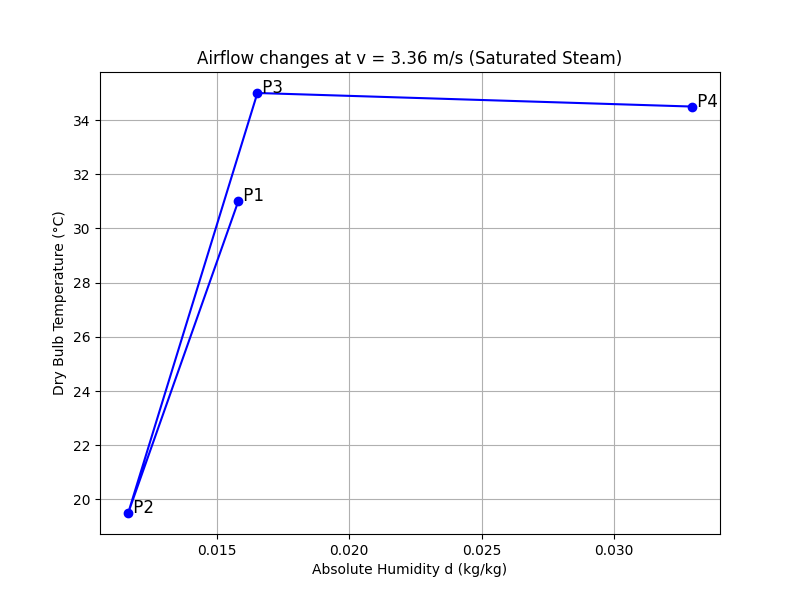
\includegraphics[width=\linewidth]{Plots/sat_v_3_36.png}
        \caption{Saturated, v = 3.36 m/s}
    \end{subfigure}
    \hfill
    \begin{subfigure}{0.48\textwidth}
        \centering
        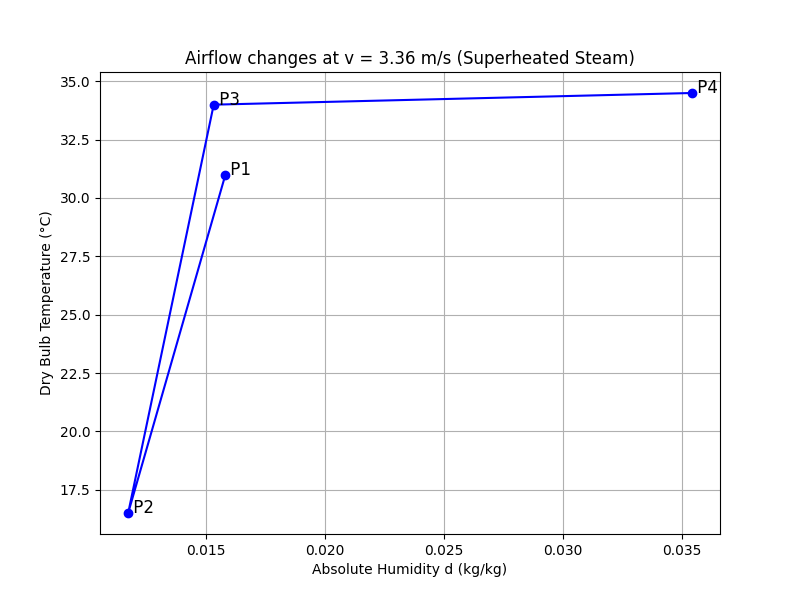
\includegraphics[width=\linewidth]{Plots/sup_v_3_36.png}
        \caption{Superheated, v = 3.36 m/s}
    \end{subfigure}
    
    \vspace{0.5cm}
    \begin{subfigure}{0.48\textwidth}
        \centering
        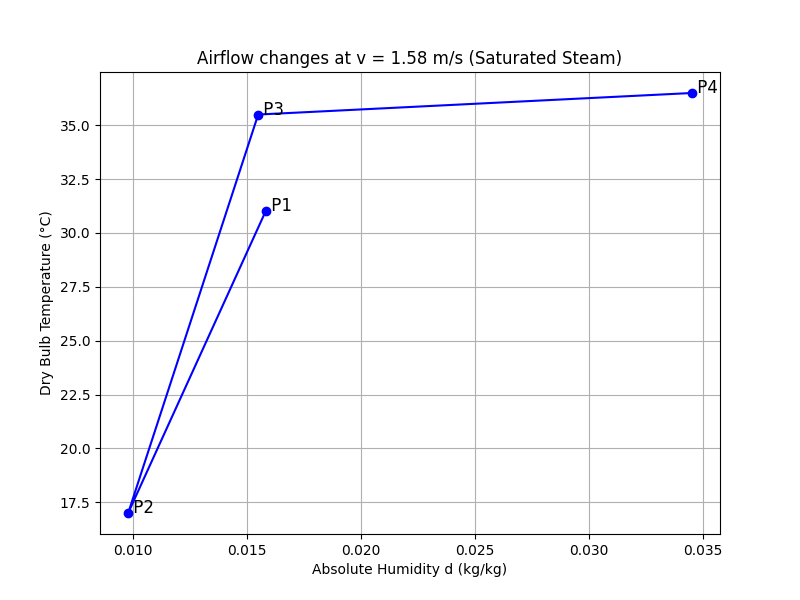
\includegraphics[width=\linewidth]{Plots/sat_v_1_58.png}
        \caption{Saturated, v = 1.58 m/s}
    \end{subfigure}
    \hfill
    \begin{subfigure}{0.48\textwidth}
        \centering
        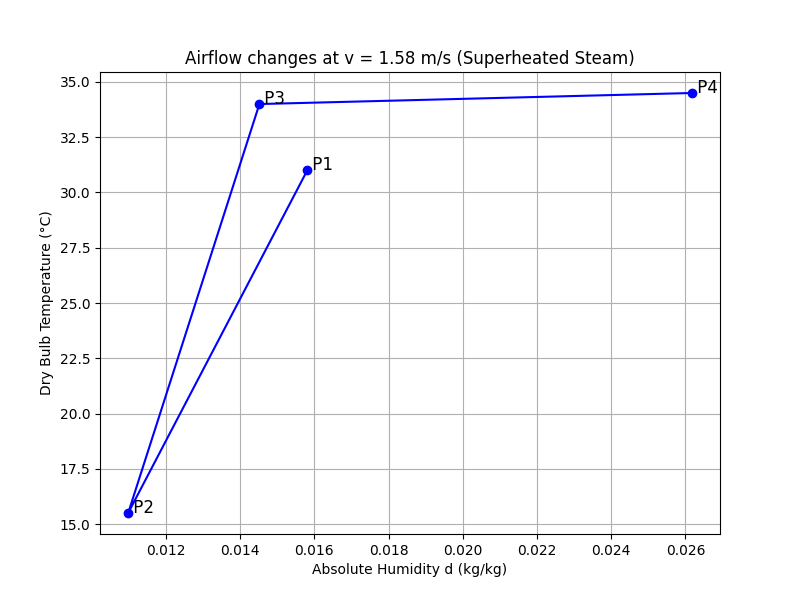
\includegraphics[width=\linewidth]{Plots/sup_v_1_58.png}
        \caption{Superheated, v = 1.58 m/s}
    \end{subfigure}
    
    \vspace{0.5cm}
    \begin{subfigure}{0.48\textwidth}
        \centering
        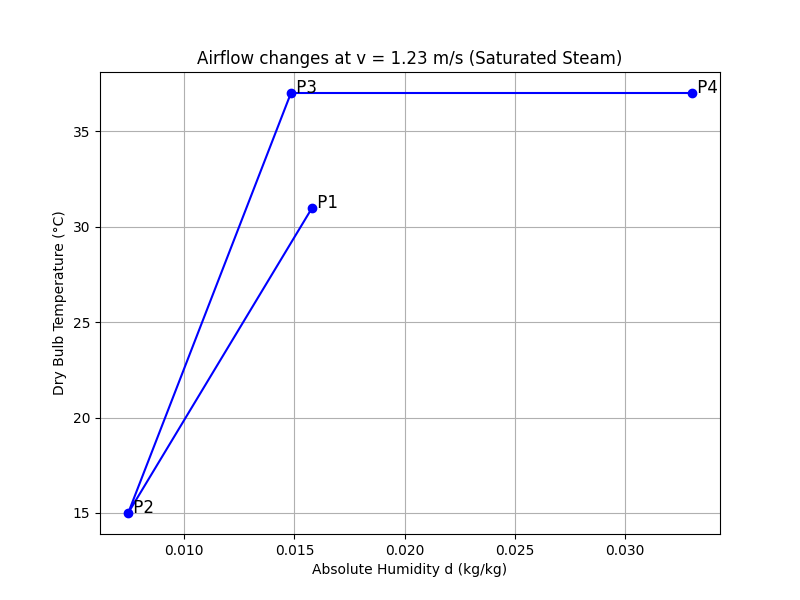
\includegraphics[width=\linewidth]{Plots/sat_v_1_23.png}
        \caption{Saturated, v = 1.23 m/s}
    \end{subfigure}
    \hfill
    \begin{subfigure}{0.48\textwidth}
        \centering
        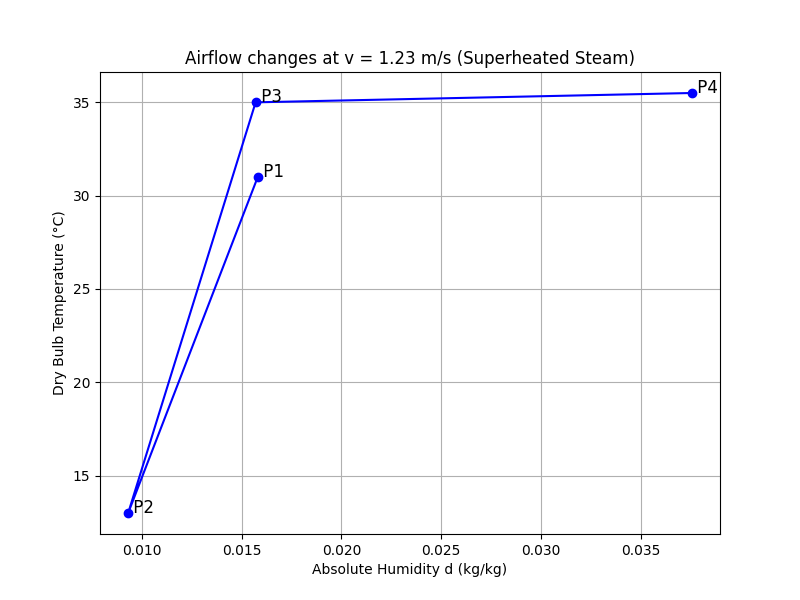
\includegraphics[width=\linewidth]{Plots/sup_v_1_23.png}
        \caption{Superheated, v = 1.23 m/s}
    \end{subfigure}
    
    \caption{Psychrometric Process Change for Different Airflows}
\end{figure}
